% Author: Izaak Neutelings (June 2017)
\documentclass[border=3pt,tikz]{standalone}
\usepackage{amsmath} % for \text
\tikzset{>=latex} % for LaTeX arrow head
%\usetikzlibrary{patterns} % for hatches area

% colors
\definecolor{mylightred}{RGB}{255,200,200}
\definecolor{mylightblue}{RGB}{172,188,63}
\definecolor{mylightgreen}{RGB}{150,220,150}

\def\tick#1#2{\draw[thick] (#1) ++ (#2:0.015) --++ (#2-180:0.03)}

\begin{document}


% ISOLATION REGIONS 1
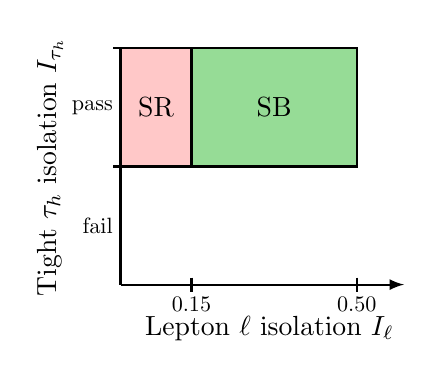
\begin{tikzpicture}[scale=6]
  
  % define to change easily
  \def\isolep{0.15}
  \def\isotauM{0.10} % medium
  \def\isotauM{0.10} % loose
  \def\isoSB{0.50}
  \def\isomax{0.60}
  \def\ymax{0.50}
  
  % axes
  \draw[thick]
    (0,0) -- (0,\ymax)
    node[midway,rotate=90,above=17pt] {Tight $\tau_h$ isolation $I_{\tau_h}$};
  \draw[->,thick]
    (0,0) -- (\isomax,0)
    node[at end,below=16pt,left] {Lepton $\ell$ isolation $I_\ell$};
  
  % boxes
  \draw[thick,fill=mylightgreen]
    (\isolep,\ymax) rectangle (\isoSB,\ymax/2)
    node[midway] {SB};
  \draw[thick,fill=mylightred]
    (0,\ymax) rectangle (\isolep,\ymax/2)
    node[midway] {SR};
  
  % labels
  \node[left,scale=0.8] at (0,1*\ymax/4) {fail};
  \node[left,scale=0.8] at (0,3*\ymax/4) {pass};
  \tick{0,\ymax/2}{0};
  \tick{0,\ymax}{0};
  \tick{\isolep,0}{90} node[below=-1,scale=0.8] {$\isolep$};
  \tick{\isoSB,0}{90} node[below=-1,scale=0.8] {$\isoSB$};
  
\end{tikzpicture}


% ISOLATION REGIONS 2
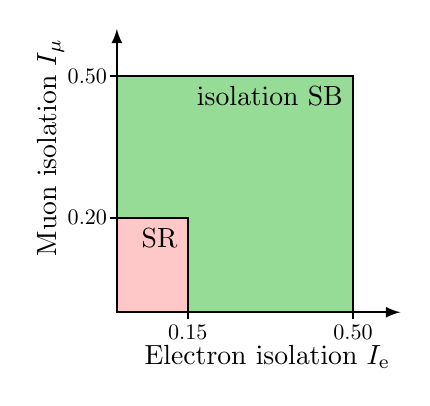
\begin{tikzpicture}[scale=6]
  
  % define to change easily 
  \def\isoe{0.15}
  \def\isomu{0.20}
  \def\isoSB{0.50}
  \def\isomax{0.60}
  
  % axes
  \draw[->,thick]
    (0,0) -- (0,\isomax)
    node[at end,left=24pt,rotate=90] {Muon isolation $I_\mu$};
  \draw[->,thick]
    (0,0) -- (\isomax,0)
    node[at end,below=16pt,left] {Electron isolation $I_\text{e}$};
  
  % boxes
  \draw[thick,fill=mylightgreen]
    (0,0) rectangle (\isoSB,\isoSB)
    %(0,\isomu) rectangle (\isoSB,\isoSB)
    node[anchor=north east] {isolation SB};
  \draw[thick,fill=mylightred]
    (0,0) rectangle (\isoe,\isomu)
    node[anchor=north east] {SR};
  
  % labels
  \tick{0,\isomu}{0} node[left=-2,scale=0.8] {$\isomu$};
  \tick{0,\isoSB}{0} node[left=-2,scale=0.8] {$\isoSB$};
  \tick{\isoe,0}{90} node[below=-1,scale=0.8] {$\isoe$};
  \tick{\isoSB,0}{90} node[below=-1,scale=0.8] {$\isoSB$};
  
\end{tikzpicture}


% CONTROL REGIONS 3
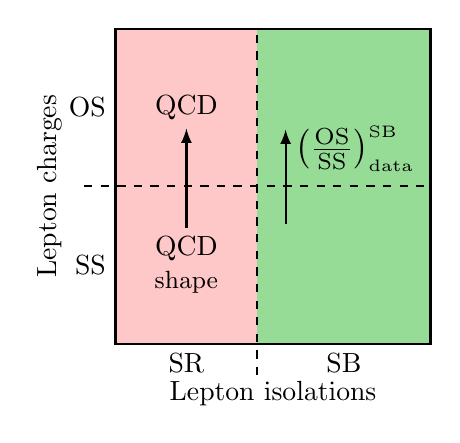
\begin{tikzpicture}[scale=4]
  
  \def\mx{0.45} %middle
  
  % boxes
  \fill [mylightred] % SR
    (0,0) rectangle (\mx,1);
  \fill [mylightgreen] % SB
    (\mx,0) rectangle (1,1);
  \draw[thick]
    (0,0) rectangle (1,1);
  
  % dashed lines
  \draw[dashed,thick]
    (\mx,-0.1) -- (\mx,1);
  \draw[dashed,thick]
    (-0.1,0.5) -- (1,0.5);
  
  % labels
  \draw
    (0,0.75) node[anchor=east]  {OS}
    (0,0.25) node[anchor=east]  {SS}
    (\mx/2,0) node[anchor=north] {SR}
    (0.5+\mx/2,0) node[anchor=north] {SB}
    (0,0.50) node[rotate=90,above=16pt] {Lepton charges}
    (0.50,0) node[below=10pt] {Lepton isolations};
  \node[align=center,scale=1,inner sep=3] (SB) at (\mx/2,0.25) {QCD\\\small shape};
  \node[align=center,scale=1,inner sep=3] (SR) at (\mx/2,0.75) {QCD};
  
  % arrows
  \draw[->,thick] % SB: SS -> OS
    (SB) -- (SR);
  \draw[->,thick] % SB: SS -> OS
    (1.2*\mx,0.38) --++ (0,0.3)
    node[pos=0.8,right=-1,scale=1.2]{$\left(\frac{\text{OS}}{\text{SS}}\right)^\text{\tiny SB}_\text{\tiny data}$};
  
\end{tikzpicture}


% CONTROL REGIONS 4
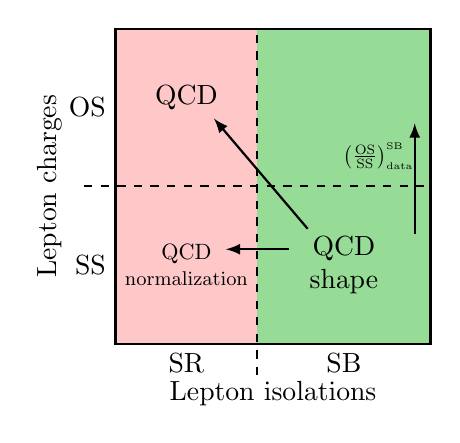
\begin{tikzpicture}[scale=4]
  
  \def\mx{0.45} %middle
  
  % boxes
  \fill [mylightred] % SR
    (0,0) rectangle (\mx,1);
  \fill [mylightgreen] % SB
    (\mx,0) rectangle (1,1);
  \draw[thick]
    (0,0) rectangle (1,1);
  
  % dashed lines
  \draw[dashed,thick]
    (\mx,-0.1) -- (\mx,1);
  \draw[dashed,thick]
    (-0.1,0.5) -- (1,0.5);
  
  % labels
  \draw
    (0,0.75) node[anchor=east]  {OS}
    (0,0.25) node[anchor=east]  {SS}
    (\mx/2,0) node[anchor=north] {SR}
    (0.5+\mx/2,0) node[anchor=north] {SB}
    (0,0.50) node[rotate=90,above=16pt] {Lepton charges}
    (0.50,0) node[below=10pt] {Lepton isolations};
  \draw
    (\mx/2,0.78) node {QCD}
    (0.5+\mx/2,0.25) node[align=center] {QCD\\shape} %{$\text{QCD}^\text{SS,SB}_\text{data}$};
    (\mx/2,0.25) node[align=center,scale=0.80] {QCD\\\small normalization};
  
  % arrows
  \draw[->,thick] % SR: SS -> OS
    (\mx+0.1,0.30) -- (\mx-0.1,0.30);
    %node[midway,above=8pt,right=-2pt,scale=0.70]{};
  \draw[->,thick] % SB: SS -> OS
    (0.95,0.35) -- (0.95,0.7)
    node[midway,above=8pt,left=-2pt,scale=0.70]{$\left(\frac{\text{OS}}{\text{SS}}\right)^\text{\tiny SB}_\text{\tiny data}$};
  
  \begin{scope}[shift={(\mx+0.02,0.54)},scale=0.35]
    \draw[->,thick]
      (0.40,-0.5) -- (-0.45,0.5);
      %node[midway,above=5pt,right=0pt,scale=0.8]{ $F^{\tiny \text{e}\mu}_\text{\tiny sim}$};
  \end{scope}
  
\end{tikzpicture}


\end{document}